
\newcolumntype{R}[1]{>{\raggedleft\arraybackslash}p{#1}}
\newcolumntype{L}[1]{>{\raggedright\arraybackslash}p{#1}}

\newcommand{\MyDiamond}[1][fill=black]{
\begin{tikzpicture}[x=1.2ex,y=1.2ex,line width=.1ex,line join=round, yshift=0.0ex] \draw  [#1]  (0,.5) -- (.5,1) -- (1,.5) -- (.5,0);
\end{tikzpicture}
}

\newcommand{\MyPlus}[1][fill=black]
{
\begin{tikzpicture}[x=1.5ex,y=1.5ex,line width=0.5ex]
\draw[#1] (0,.5) -- (1,.5);
\draw[#1] (.5,0) -- (.5,1);
\end{tikzpicture}
}

\newcommand{\MyCross}[1][fill=black]
{
\begin{tikzpicture}[x=1.ex,y=1.ex,line width=0.5ex]
\draw[#1] (0,0) -- (1,1);
\draw[#1] (0,1) -- (1,0);
\end{tikzpicture}
}

\newcommand{\MyTriangle}[1][fill=black]
{
\begin{tikzpicture}[x=1.ex,y=1.ex,line width=0.2ex]
\draw[#1] (0,1) -- (1,1);
\draw[#1] (1,1) -- (.5,0);
\draw[#1] (.5,0) -- (0,1);
\fill[#1] (0,1) -- (1,1) -- (.5,0) -- cycle;
\end{tikzpicture}
}

\newcommand{\MySolidLine}[1][fill=black]
{
\begin{tikzpicture}[x=2.ex,y=1.ex,line width=0.5ex]
\draw[#1] (0,.5) -- (2.5,.5);
\end{tikzpicture}
}

\newcommand{\MyDashedLine}[1][fill=black]
{
\begin{tikzpicture}[x=2.ex,y=1.ex,line width=0.5ex]
\draw [#1,dashed] (0,.5) -- (2.5,.5);
\end{tikzpicture}
}

\newcommand{\MyDashedDottedLine}[1][fill=black]
{
\begin{tikzpicture}[x=2.ex,y=1.ex,line width=0.5ex]
\draw [#1,dash dot] (0,.5) -- (2.5,.5);
\end{tikzpicture}
}

\newcommand{\MyDottedLine}[1][fill=black]
{
\begin{tikzpicture}[x=2.ex,y=1.ex,line width=0.5ex]
\draw [#1,dotted] (0,.5) -- (2.5,.5);
\end{tikzpicture}
}

\chapter{Test problems}
\label{c:test-problems}
To understand how evolving the total energy density may deteriorate simulation results and to demonstrate how much the new scheme improves, we compare the results from evolving $E$ by the flux $M$ (original scheme) with that from evolving $\tilde{E}$ by the flux $(\tilde{E}+p)U_{x}/\gamma$ (new scheme). Since catastrophic cancellation is likely to occur in UR and NR limits, we will conduct several test problems in these two limits. All simulations throughout this paper adopt the HLLC Riemann solver and PLM data reconstruction unless otherwise specified.

\definecolor{NewHot}{RGB}{255, 216, 23}
\definecolor{NewCold}{RGB}{21, 143, 191}
\definecolor{OriHot}{RGB}{158,54,86}
\definecolor{OriCold}{RGB}{204, 149, 47}
\section{Convergence test for sinusoidal waves}
\label{section:convergence test}
We perturb proper mass density in the high- and low-$T$ limits to compare the accuracy of both schemes over a wide dynamical range. We construct the initial conditions as follows. All cases share homogeneous and static background with proper mass density $\rho_{0}=1$ on uniform grids, whereas the ambient temperatures are set to $k_{B}T/mc^2=10^{10}$ and $10^{-10}$ for the high- and low-$T$ limits, respectively. We then sinusoidally perturb the background with a tiny amplitude, $\delta \rho/\rho_{0}=10^{-6}$.

To monitor how errors in the numerical solution decrease as a function of increasing spatial resolution in the three-dimensional space, we adopt a propagating wave along the diagonal direction of the simulation cubic box with the periodic boundary condition. Thus, the analytical solution is $\rho(\mathbf{x},t)=\rho_{0}+\delta\rho\sin \left[\left(x+y+z\right)/\sqrt{3}-c_{s}t\right]$, where $c_{s}$ is the sound speed given by Equation~(\ref{sound_speed}).

We define the L1-norm error as
\begin{equation}
L1(Q)=\frac{1}{N}\sum^{N}_{i=1}\abs{1-\frac{Q_{\text{numerical}}\left(\mathbf{x_{i}}\right)}{Q_{\text{analytical}}\left(\mathbf{x_{i}}\right)}},
\label{relative L1 error}
\end{equation}
where $Q_{\text{numerical}}\left(\mathbf{x_{i}}\right)$ is the numerical solution of $i$-th cell at $\mathbf{x_{i}}$ and $Q_{\text{analytical}}\left(\mathbf{x_{i}}\right)$ is the corresponding analytical solution.
We then calculate the L1 error of the proper mass density along the wave propagating direction.
As shown in \Cref{fig:convergence test}, the L1 errors of the new scheme in both the high-$T$ limit ($\tikz\draw[black,fill=NewHot] (0,0) rectangle (0.15,0.15);$) and low-$T$ limit ($\MyPlus[draw=NewCold,fill=NewCold]$) decrease as $N^{-2}$, consistent with the second-order accuracy of the MUSCL-Hancock scheme with PLM data reconstruction. However, the error of the original scheme in the low-$T$ limit (\tikz\draw[black,fill=OriCold] (0,0) circle (.5ex);) is much larger and roughly equal to a constant of $2\times 10^{-6}$. This is expected because the error arising from the original scheme can be estimated from \Cref{eq:OriRelativeError} in the NR limit:
\begin{equation}
    \frac{4}{3\left(\frac{k_{B}T}{mc^2}\right)}\epsilon_{\text{machine}},
    \label{eq:error in the NR limit}
\end{equation}
where $k_{B}T/mc^2=10^{-10}$ and $\epsilon_{\text{machine}}\sim 10^{-16}$ for double precision.

We thus conclude that for the original scheme in the NR limit, the cancellation between $(E/Dc^2)^2$ and $[(\abs{\mathbf{M}}/Dc)^2+1]$ leads to an error of $\sim 10^{-6}$ when computing primitive variables, roughly consistent with the L1 error (\tikz\draw[black,fill=OriCold] (0,0) circle (.5ex);). For the opposite high-$T$ limit ($\MyDiamond[draw=black,fill=OriHot]$), the discretization error, however, completely overwhelms the error ($\sim 4\epsilon_{\text{machine}}\sim4\times 10^{-16}$) estimated from \Cref{eq:OriRelativeError} in the high-$T$ limit, thus dominating the L1 error. The error arising from the cancellation in the new scheme, $\left(\tilde{E}/Dc^2\right)^2+2\left(\tilde{E}/Dc^2\right)-\left(\abs{\mathbf{M}}/Dc\right)^2$, on the left side of \Cref{transcendental equation}, is close to $\epsilon_{\text{machine}}$ in both the high- and low-$T$ limits when $\mathscr{M}<1$ (see Section \ref{section: Conversion between primitive variables and conserved ones} and Appendix \ref{Appendix:Numerical error analysis} for details).



\section{1-D relativistic Riemann problems}
\label{subsec:1-DReletivisticRiemann problems}
The 1-D Riemann problem \citep{SOD1978} has played an important role by providing exact nonlinear solutions against which (relativistic) hydrodynamic codes can be tested. Riemann problem is an initial-value problem with a piece-wise constant initial data that has a single discontinuity in the domain of interest. In this section, we directly compare the new and original schemes by simulating two relativistic Riemann problems. We then demonstrate that the new scheme handles both the UR and NR limits very well. By contrast, the original scheme severely suffers from numerical errors in the NR limit. Both schemes share the same numerical setup, e.g., MUSCL-Hancock integration, PLM data reconstruction, hybrid van-Leer, generalized minmod slope limiter, and uniform grids with the outflow boundary condition. In addition, we have numerically derived the exact solution of a nontrivial relativistic Riemann problem with the TM EoS (see Appendix \ref{appendix:exact solution} for details) in order to verify the numerical results.


\begin{table*}[t]
\caption{The left and right initial states of the Riemann problems in Section \ref{subsec:1-DReletivisticRiemann problems}. We denote the left/right states by the subscript $L/R$.}
\label{tb:IC_RiemannProblems}
\begin{tabular}{@{}lrrrrrrr@{}}
\hline
                         & $p_{L}$   & $\rho_{L}$ & $U_{L}$   & $p_{R}$    & $\rho_{R}$ & $U_{R}$   & Floating-point format \\ \hline
Ultra-relativistic limit & $1.0$     & $10^{-5}$  & $10^6$    & $1.0$      & $10^{-5}$  & $-10^{6}$ & Double precision      \\ \hline
Mixed limits             & $10^{-4}$ & $10^{2}$   & $10^{-3}$ & $10^{-10}$ & $10^{-12}$ & $-10^{2}$  & Single precision      \\ \hline
\end{tabular}
\end{table*}

\definecolor{HeadOnCollisionExact}{RGB}{122, 24, 18}
\definecolor{HeadOnCollisionOri}{RGB}{179, 169, 62}
\definecolor{HeadOnCollisionNew}{RGB}{69, 177, 230}

\section{Ultra-relativistic limit}
\label{subsubsec:Ultra-relativistic limit}
We simulate a head-on collision of two identical gases with $\gamma=10^{6}$ and $k_{B}T/mc^2=10^5$ with uniform 512 grids. The computational domain is in the interval $[0,1]$. The initial discontinuity is located at $x=0.5$. The first row of Table~\ref{tb:IC_RiemannProblems} presents the initial right and left states. \Cref{fig:head-on collision shock tube} shows the results at $t=1.0$. The left panels show the entire simulation domain, while the right panels show the zoom-in image of the post-shock region, which has been violently heated up to ultra-relativistically hot temperature ($k_{B}T/mc^2 \sim 10^{11}$) by the extremely high-$\gamma$ gases flowing inwards from both sides. As can be seen, the new scheme ($\tikz\draw[HeadOnCollisionNew,fill=white,line width=1] (0,0) circle (.5ex);$) fully agrees with the original scheme ($\MyCross[draw=HeadOnCollisionOri,fill=HeadOnCollisionOri]$) on the large-scale profile but also on the small-scale errors, meaning that the new scheme does not sacrifice the numerical accuracy in the UR limit. In addition, we notice that the non-negligible and spurious waves occur in the post-shock region, which are not due to root-finding iterations but to spatial discretization errors as the spurious waves can be reduced by increasing spatial resolution.


\begin{figure*}
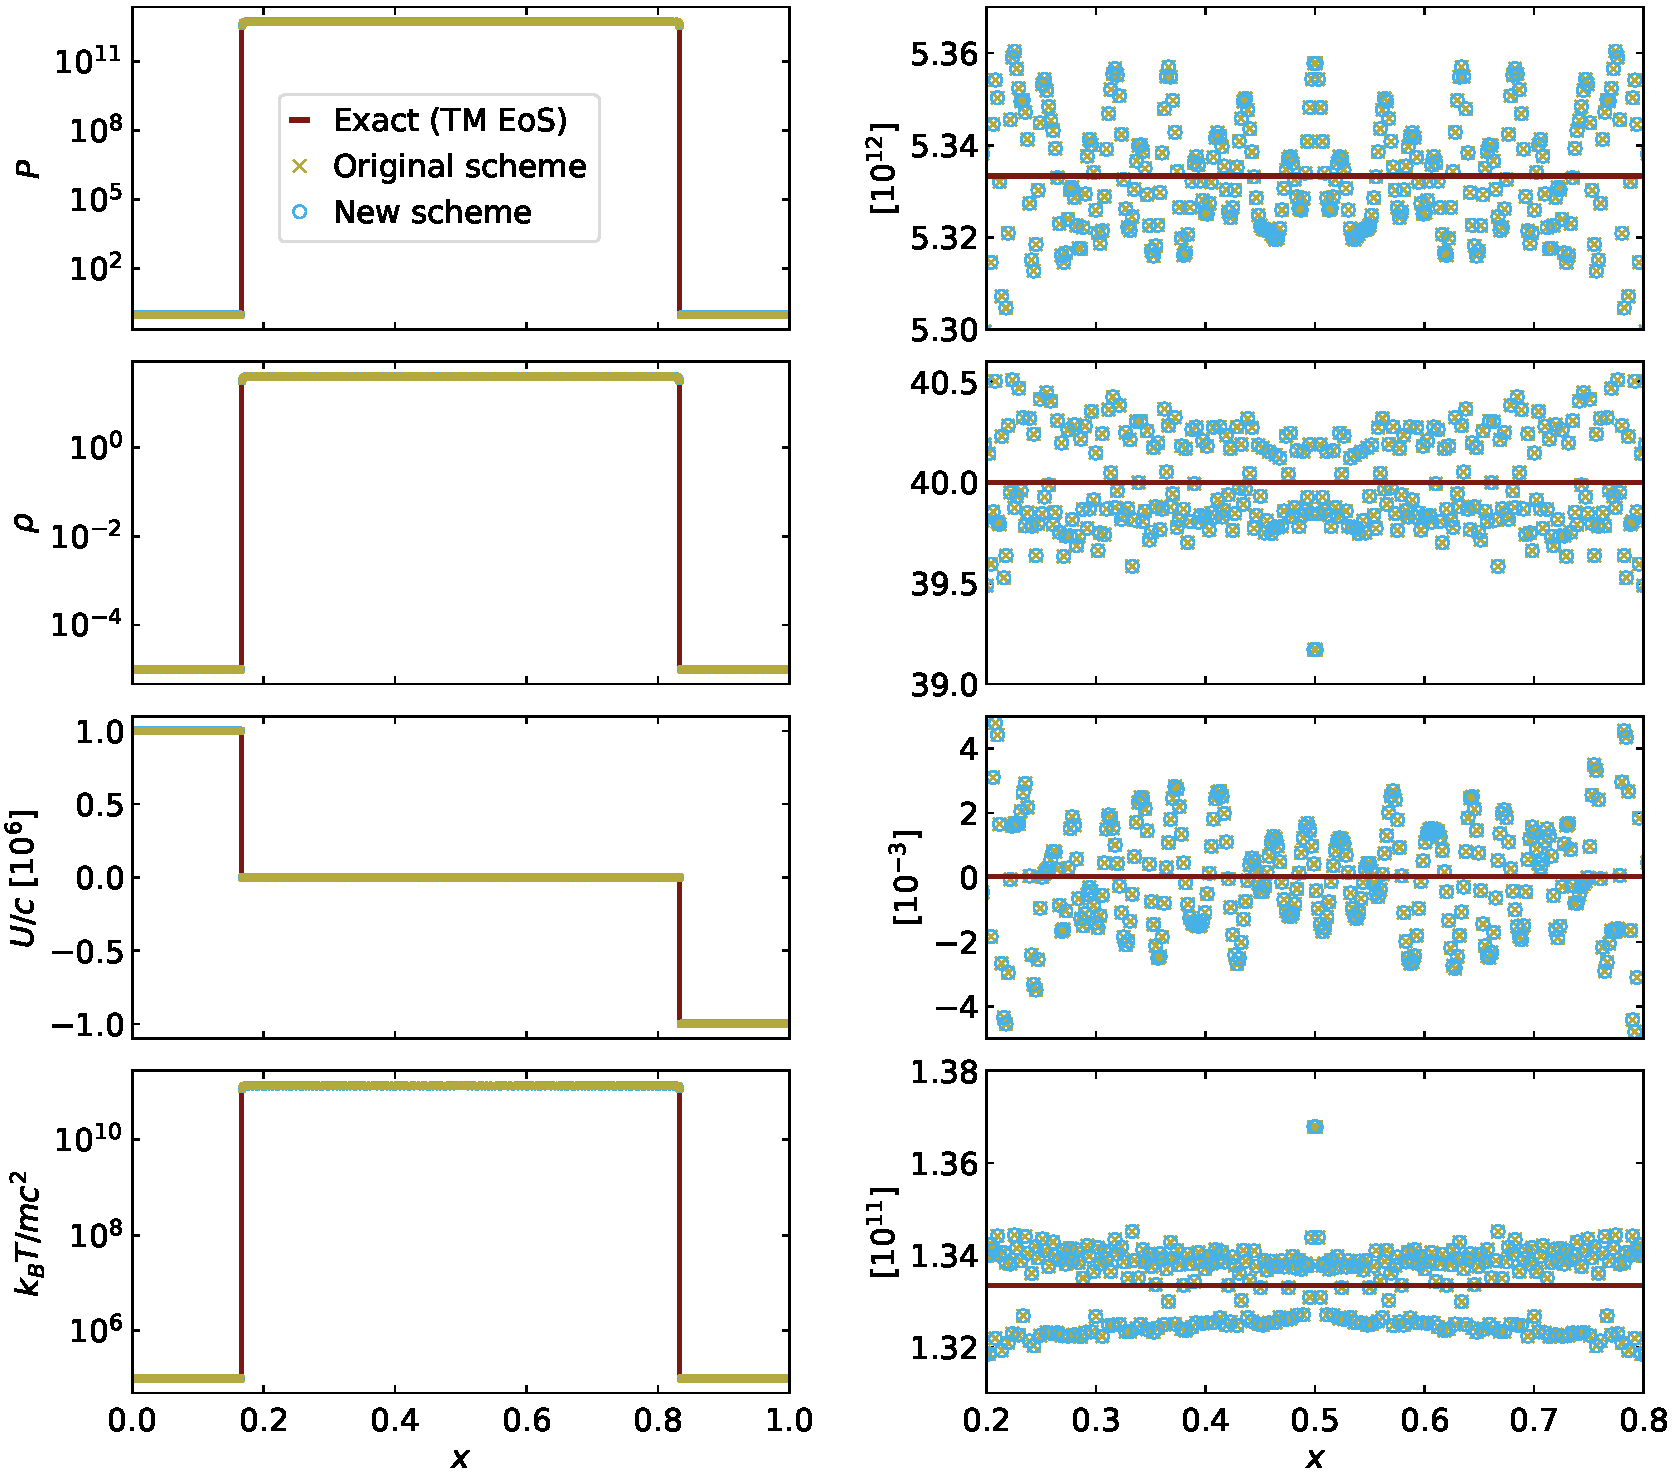
\includegraphics[width=\linewidth]{figures/HeadCollision.pdf}
\caption{Riemann problem in the UR limit with a head-on collision of two identical gases with $\beta\gamma=10^{6}$ and $k_{B}T/mc^2=10^{5}$ at $t=1.0$. The left column shows the entire simulation domain, while the right column shows the zoom-in image of the post-shock region. From top to bottom: pressure, proper mass density, four-velocity, and temperature. Note that we plot the Mach number in the zoom-in image (right column) of four-velocity so as to readily compare the amplitude of velocity oscillation with sound speed. The new scheme (blue circles) fully agrees with the original scheme (olive crosses) not only on the large-scale profiles but also on the small-scale errors, meaning that the new scheme (blue circles) does not sacrifice (or improve) the numerical accuracy in the UR limit for  that in the NR limit.}
\label{fig:head-on collision shock tube}
\end{figure*}

\definecolor{MixedLimitsOri}{RGB}{0,0,0}
\definecolor{MixedLimitsExact}{RGB}{224, 168, 0}
\definecolor{MixedLimitsNew}{RGB}{255, 20, 0}
\definecolor{MixedLimitsExactNR}{RGB}{0, 21, 255}
\definecolor{MixedLimitsExactUR}{RGB}{0, 166, 28}

\section{Mixed limits}
\label{section:NRLimit}
To demonstrate that the new scheme can handle a large dynamical range covering both extremely hot and extremely cold gases, we simulate a nontrivial Riemann problem where the temperature straddles between the high- and low-$T$ limits. This initial condition evolves into a cold left-traveling rarefaction wave separated by a contact discontinuity to match an extremely hot downstream of an ultra-relativistic shock traveling toward the right. Also, we have numerically derived the exact solution of this particular Riemann problem with the TM EoS (see Appendix \ref{appendix:exact solution}). The second row in \Cref{tb:IC_RiemannProblems} shows the initial left and right states. The simulation adopts a computational domain [0,100] with 102,400 cells. Since the speed of the right-traveling shock is 276 times faster than that of the left-traveling rarefaction wave, we put the initial discontinuity at $x=5\times10^{-2}$ to provide an ample space for the right-traveling shock.

\Cref{fig:non-relativistic shock tube} shows the results at $t=80$, where there are three points to be emphasized. First, we find not only that the shock front at $x=26$ is well resolved by 3--4 cells but also that the new scheme ($\MyCross[draw=MixedLimitsNew,fill=MixedLimitsNew]$) agrees well with the exact solution of the TM EoS ($\MySolidLine[draw=MixedLimitsExact,fill=MixedLimitsExact]$), as shown in all insets. Second, the L1 error, defined by \Cref{relative L1 error}, of the density profile from the original scheme ($\tikz\draw[MixedLimitsOri,fill=white,line width=1] (0,0) circle (.5ex);$) is 23 per cent within the region between the head of rarefaction wave ($x=2.67\times 10^{-2}$, the third number from top in the leftmost column of Table \ref{tb:exact solution} in Appendix \ref{appendix:exact solution}) and initial discontinuity ($x=5\times10^{-2}$), consistent with the 20 per cent error estimated by \Cref{eq:error in the NR limit} with $k_{B}T/mc^2=8\times10^{-6}$. Similar conclusions can be drawn for other physical quantities. However, in the region $5\times10^{-2}<x<0.3$ swept by the right-traveling contact discontinuity, errors of the original scheme are much larger than the estimate, which requires further investigation. Third, the solutions of the TM EoS ($\MySolidLine[draw=MixedLimitsExact,fill=MixedLimitsExact]$) match well with both $\Gamma=5/3$ ($\MyDashedLine[draw=MixedLimitsExactNR,fill=MixedLimitsExactNR]$) in the NR region ($x<0.21$) and $\Gamma=4/3$ ($\MyDashedDottedLine[draw=MixedLimitsExactUR,fill=MixedLimitsExactUR]$) in the UR region ($x>0.27$). It demonstrates the capability of capturing the transition from $\Gamma=5/3$ (for $k_{B}T/mc^2 \rightarrow 0$) to $\Gamma=4/3$ (for $k_{B}T/mc^2 \rightarrow \infty$) for the new scheme. The exact solutions of this test are shown in \Cref{tb:exact solution} in Appendix \ref{appendix:exact solution}.

\begin{figure*}
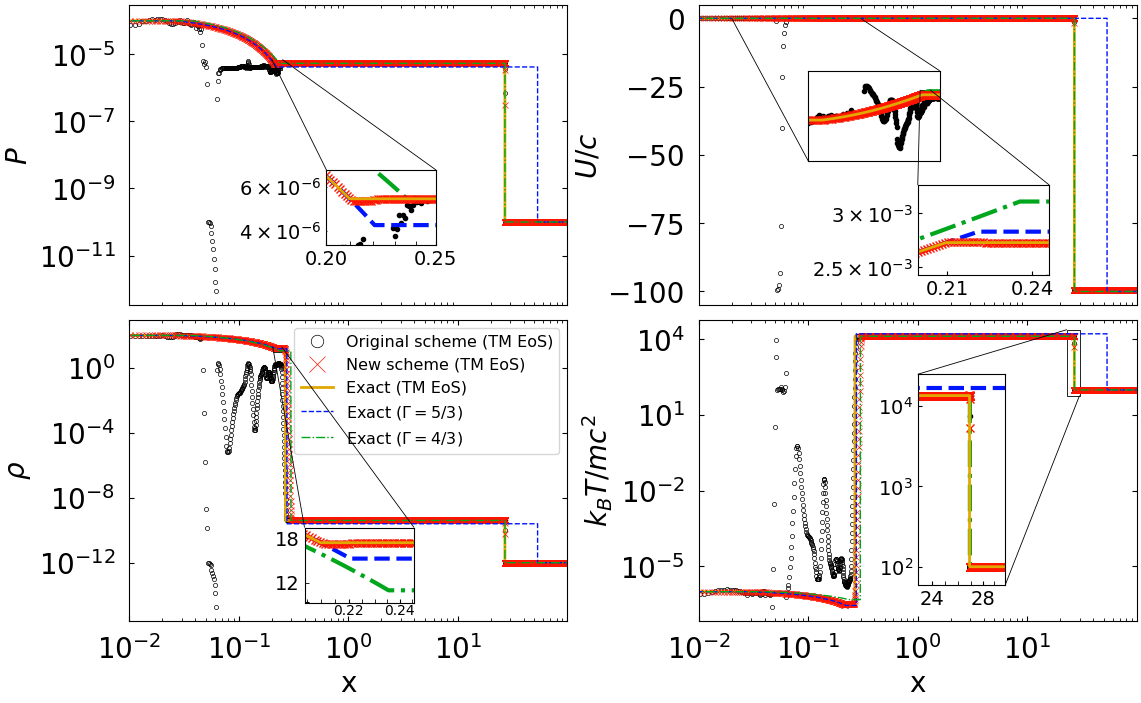
\includegraphics[width=\linewidth]{figures/RiemannProbs.png}
\centering
\caption{Riemann problem in the mixed UR and NR limits at $t=80$. The second row in Table \ref{tb:IC_RiemannProblems} shows the initial condition. Clock-wise from top-left: pressure, 4-velocity, temperature, and proper mass density. We find not only that the shock front at $x=26$ is well resolved by 3--4 cells but also that the new scheme (red crosses) agrees well with the exact solution of the TM EoS (yellow lines), as shown in all insets. The L1 error of the density profile from the original scheme (black circles) is 23 per cent within the region between the head of rarefaction wave and initial discontinuity (i.e. $2.67\times 10^{-2}<x<5\times10^{-2}$), consistent with the 20 per cent error estimated by \Cref{eq:error in the NR limit} with $k_{B}T/mc^2=8\times10^{-6}$. However, in the region $5\times10^{-2}<x<0.3$ swept by the right-traveling contact discontinuity, errors of the original scheme are much larger than the estimate, which requires further investigation. The TM profiles match well with both the $\Gamma=5/3$ profiles (blue dashed lines) in the NR region ($x<0.21$) and the $\Gamma=4/3$ profiles (green dashed lines) in the UR region ($x>0.27$).}
\label{fig:non-relativistic shock tube}
\end{figure*}

\section{Multi-dimensional grid effects for high-$\mathscr{M}$ flows}
\label{Multi-dimensional grid effects}
To investigate the detrimental impact of grid effects on the evolution of ultra-relativistic and high Mach number hydrodynamic problems, we separately simulate two identical three-dimensional mono-direction flow with different flow directions. One flow is along the diagonal direction of the simulation box and the other is parallel to the grid direction. Both simulations share the same numerical set-up as follows. Flows are initially represented by cylinders extending to the boundaries of a periodic cubic box with a width $L$. The cylinder diameter is $D=0.028L$. The proper mass density ratio of the flow and the ambient is $\rho_{\text{flow}}/\rho_{\text{amb}}=10^{-5}$. The temperatures of the flows and the ambient are $k_{B}T_{\text{flow}}/mc^2=1.0$ and $10^{-5}$, respectively. The four-velocity ($\gamma \beta$) profile inside the flow source is $10^{6}\left(1+\cos{\left(2\pi r/D\right)}\right)$, where $r$ is the distance from the flow axis inside the source. Other physical quantities are uniformly distributed inside the source.

The AMR base level is covered by $64^{3}$ cells in all cases. We adopt the gradient of the proper mass density and the magnitude of $\abs{\mathbf{M}}/D$ as the two inclusive refinement criteria. We refine a patch if the gradient of a cell satisfies
\begin{equation}
\frac{\Delta h_{\ell}}{Q}
\left(
\abs{\frac{\partial Q}{\partial x}}+
\abs{\frac{\partial Q}{\partial y}}+
\abs{\frac{\partial Q}{\partial z}}
\right)
> C_{Q},
\label{threshold for gradient}
\end{equation}
where $Q=\rho$, $C_{Q}=0.3$, and $\Delta h_{\ell}$ is the cell size at refinement level $\ell$. This criterion aims to capture the finger structure due to instabilities at the interface between the flow and the ambient gases. Also, a patch will be refined when any cell satisfies $\abs{\mathbf{M}}/D>10^{4}$ so that the high-speed region is refined to the finest level.

\Cref{fig:GridEffect} shows the simulation results at $t=0.4L/c$. In Figures \ref{fig:AAXX} and \ref{fig:DiagonalFlowLow}, we adopt four AMR levels to ensure that the flow diameter can be resolved by 28 cells. The extremely high Mach number ($\mathscr{M}\sim 10^{6}$) flow leaves any instability short of time to develop, and one expects a smooth flow-ambient interface. However, the interface of the oblique flow turns out to be subject to severe dissipation. The fuzzy-looking cross-sections in the transverse slices of the oblique flow (right column in \Cref{fig:DiagonalFlowLow}) suggest that the dissipation is caused by numerical instabilities when high Mach number flow travels obliquely across Cartesian grids. This numerical problem is not limited to relativistic high Mach number flows but also occurs in non-relativistic high Mach number flows.

To examine this issue further, we increase the spatial resolution by a factor of 2 and decrease the time-step by a factor of 0.3 from the standard Courant condition. The results (\Cref{fig:HorizontalFlowHig,fig:DiagonalFlowHig}) indicate that increasing spatial and temporal resolution can neither significantly ameliorate the dissipation nor help the oblique flow converge to the horizontal flow. This artificial grid effect can adversely influence the study of high-speed jets, especially for hydrodynamical instabilities near the jet boundaries.

An example of this boundary instability is the finger-like pattern observed immediately outside the parallel flow (right column in \Cref{fig:AAXX}), which we believe to arise from a genuine instability seeded by discritization noise. The finger-like pattern has a higher temperature than the ambient, and in fact consists of two-dimensional flat sheets along the flow. This is demonstrated in \Cref{fig:HorizontalFlowHigZoomIn} with transverse slices cut through `B' and `C'. The patterns are identical to that cut through `A' in \Cref{fig:HorizontalFlowHig}. These 2-D sheet pattern persists even after adding 1 per cent level of white noise into the background density, illustrating that the coherence of sheets along the flow direction is genuinely generated by the high-speed flow boundaries. This finger pattern is similar, but not identical, to the curvature-driven fingers of a knotted jets reported recently \citep{Gourgouliatos2017}. Our flow has a smooth and parallel boundary without any curvature to drive the fingers.

\begin{figure*}
  \centering
  \subfigure[]
    {
      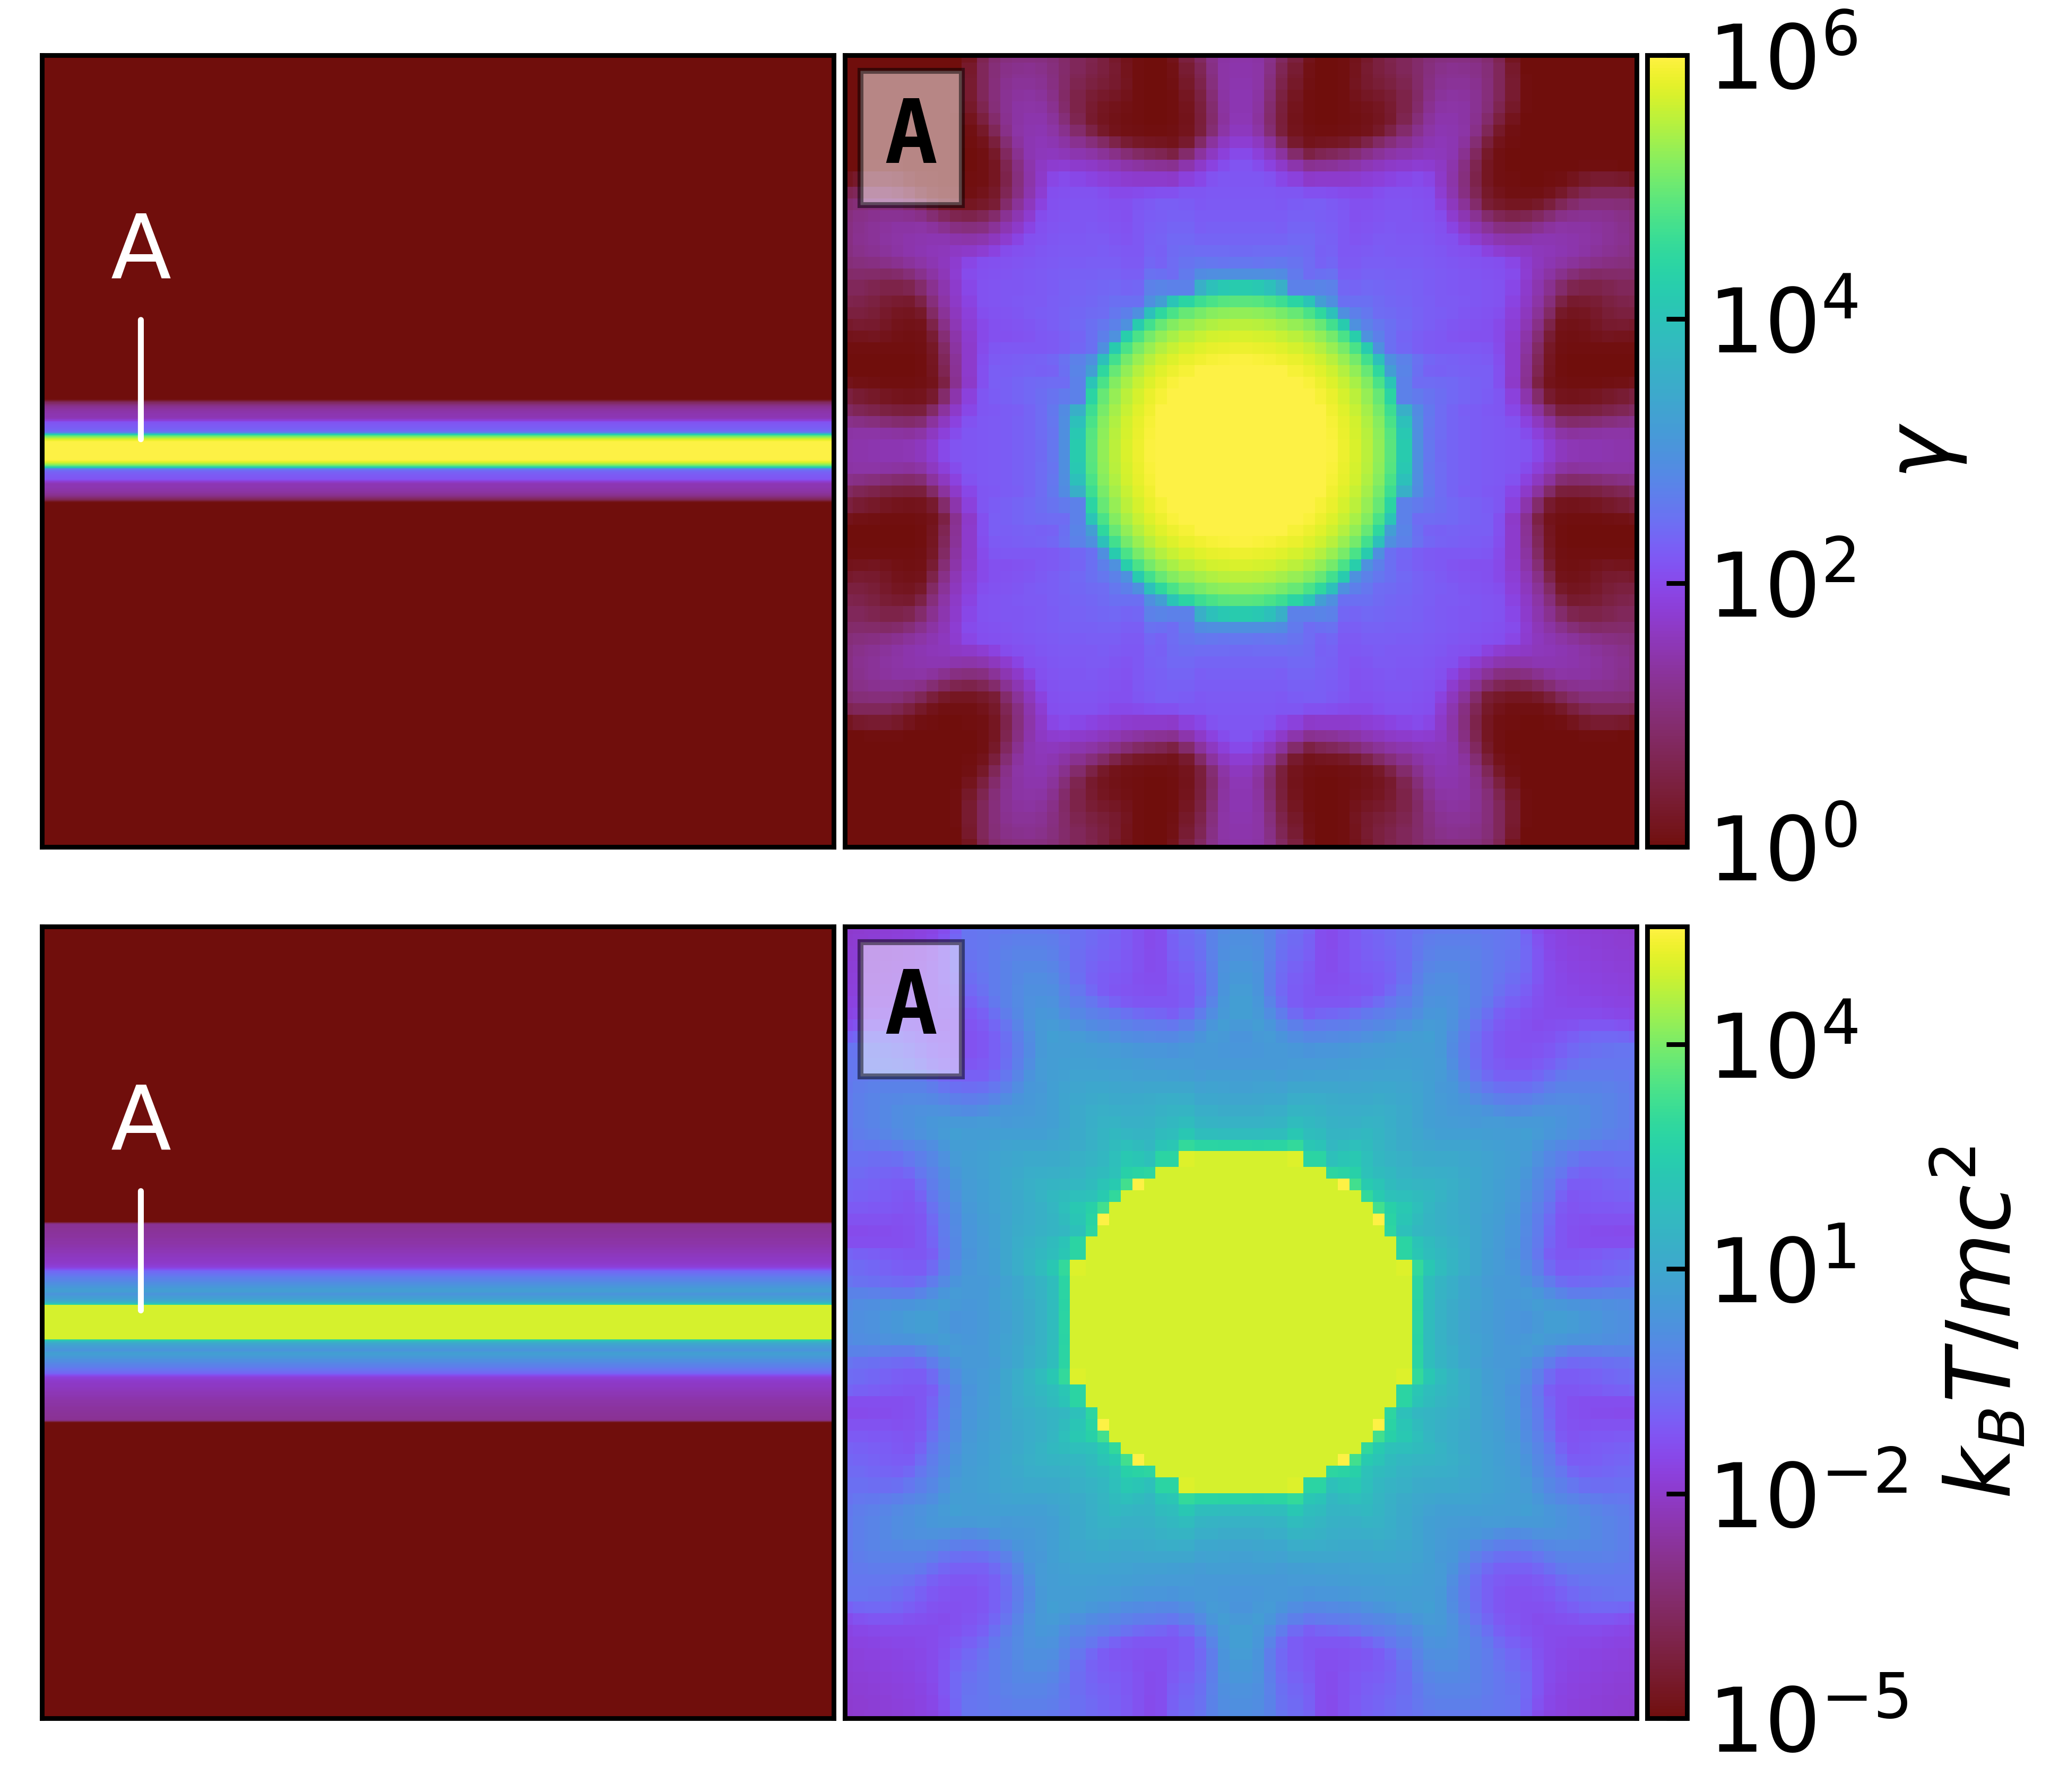
\includegraphics[width=0.45\linewidth]{figures/fig__HorizontalFlowLow.png}
      \label{fig:AAXX} % A
    }
  \subfigure[]
    {
      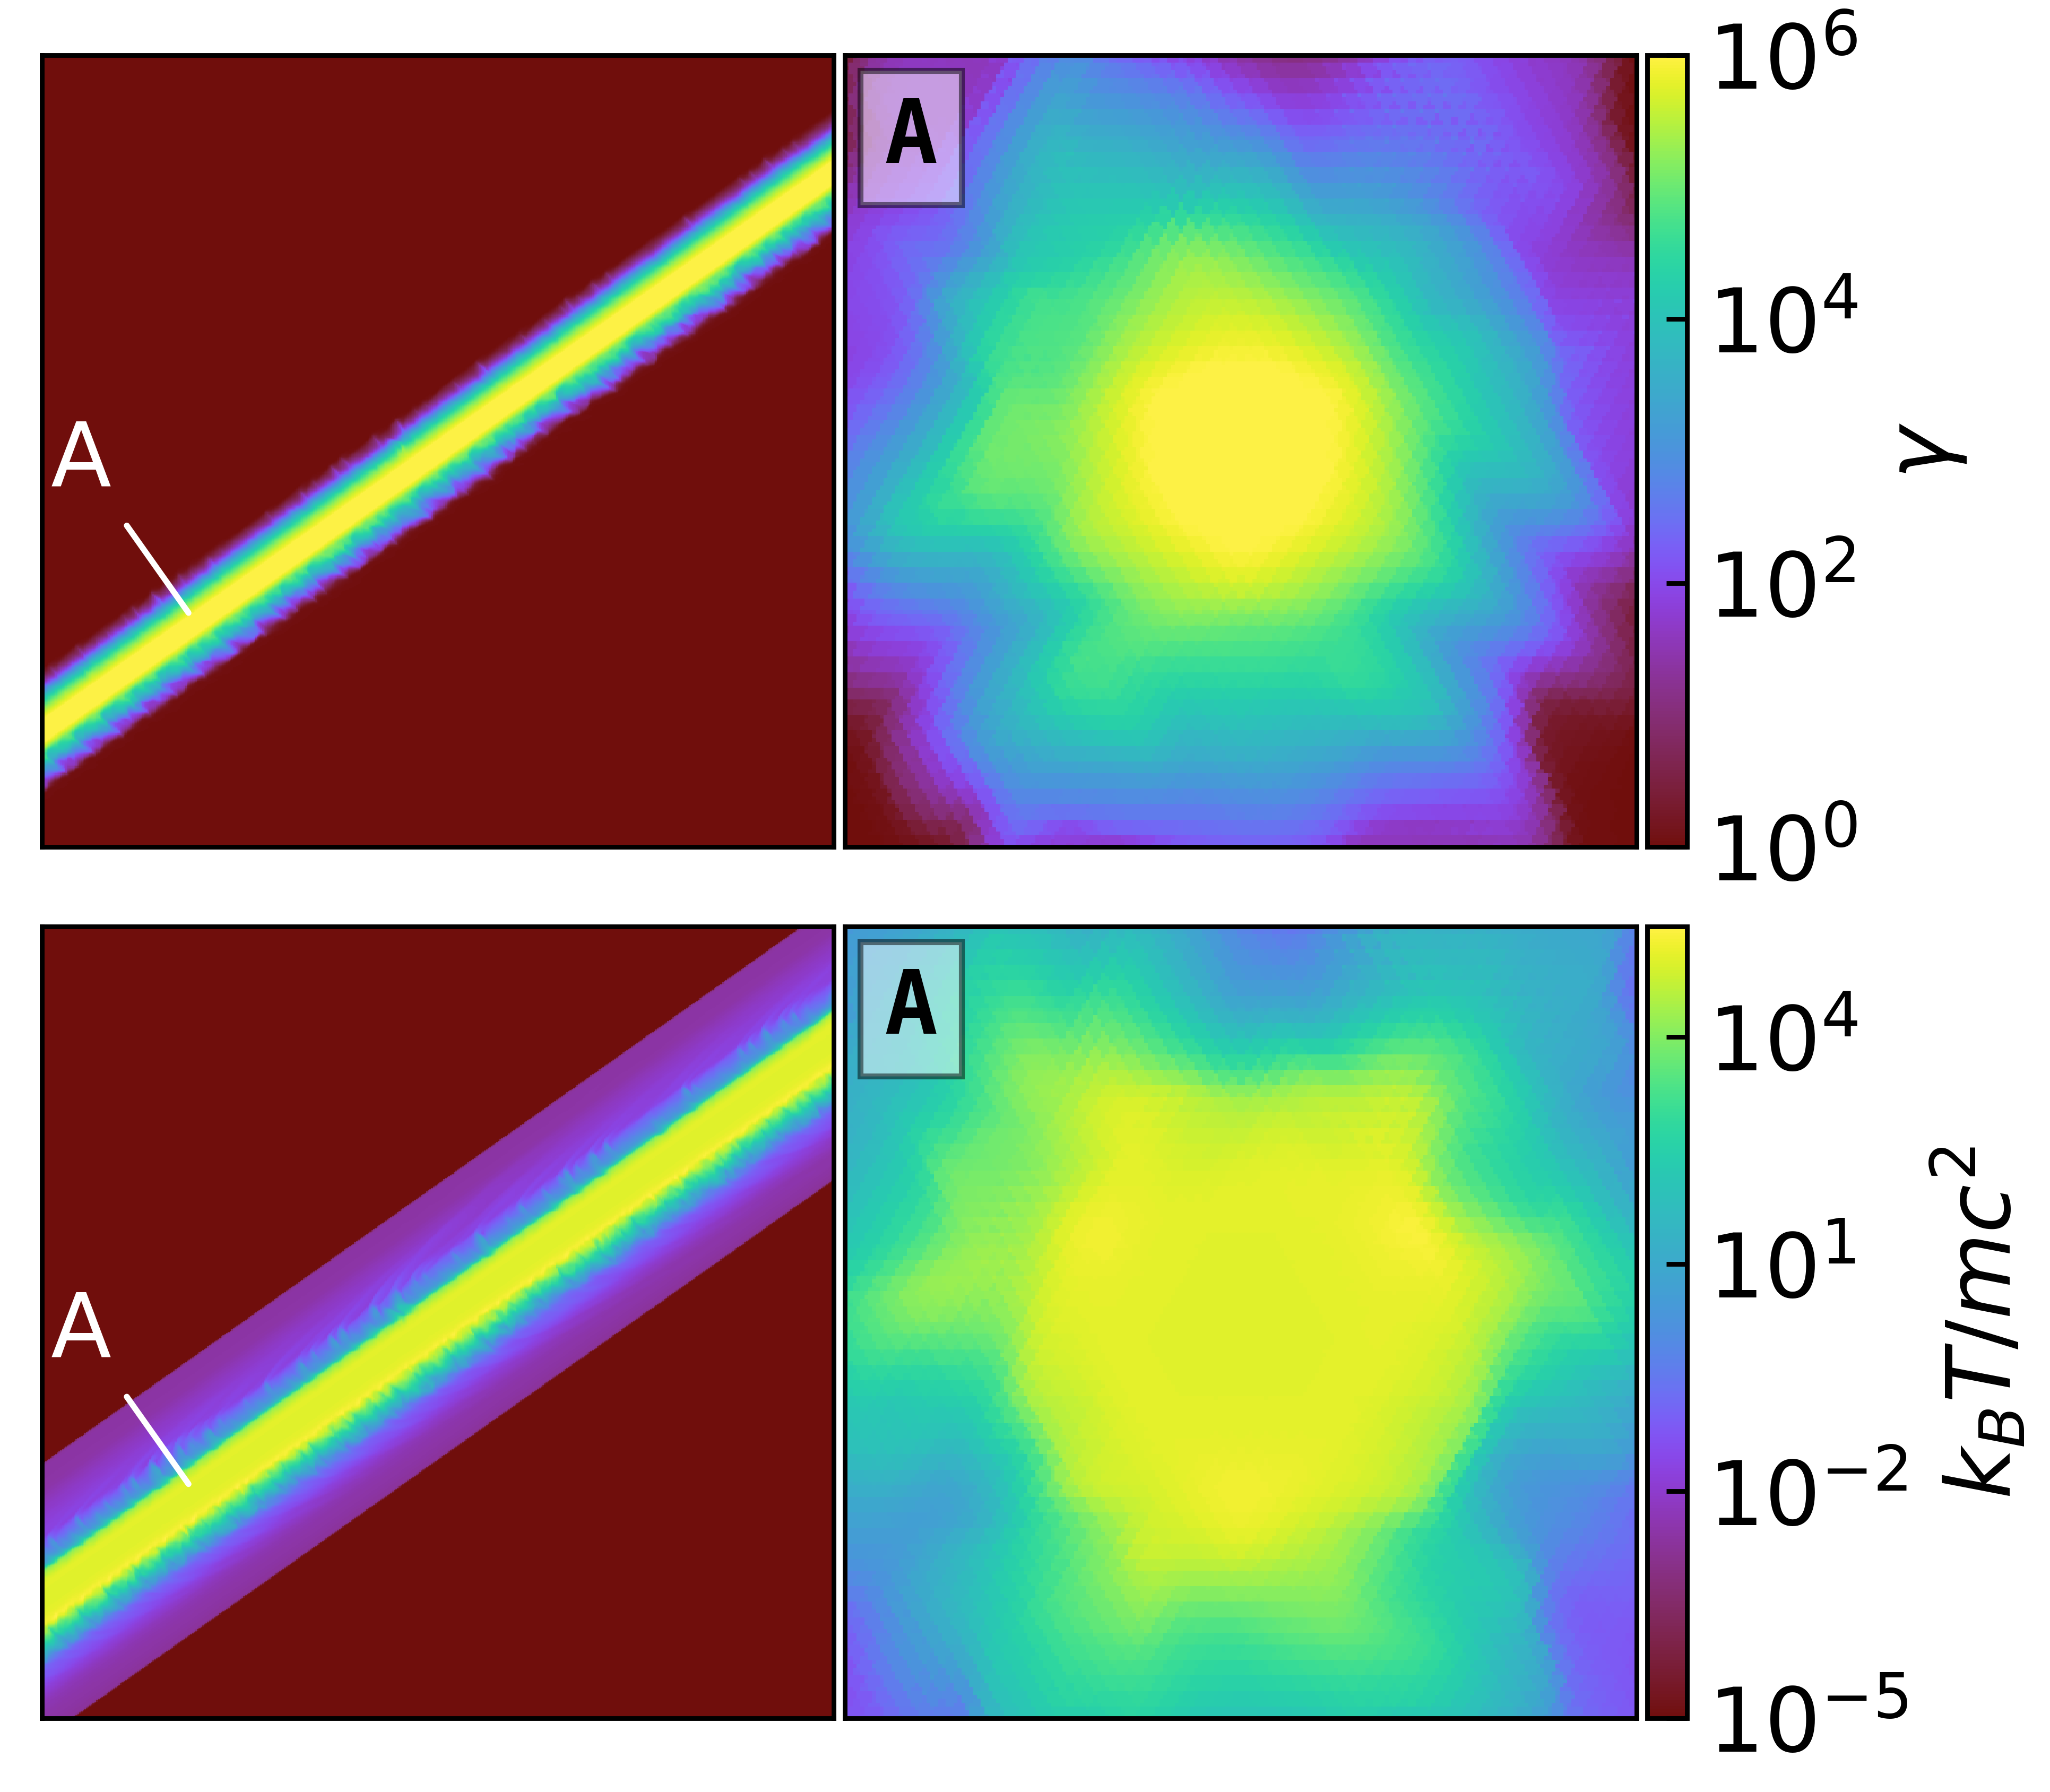
\includegraphics[width=0.45\linewidth]{figures/fig__DiagonalFlowLow.png}
      \label{fig:DiagonalFlowLow} % B
    }
  \subfigure[]
    {
      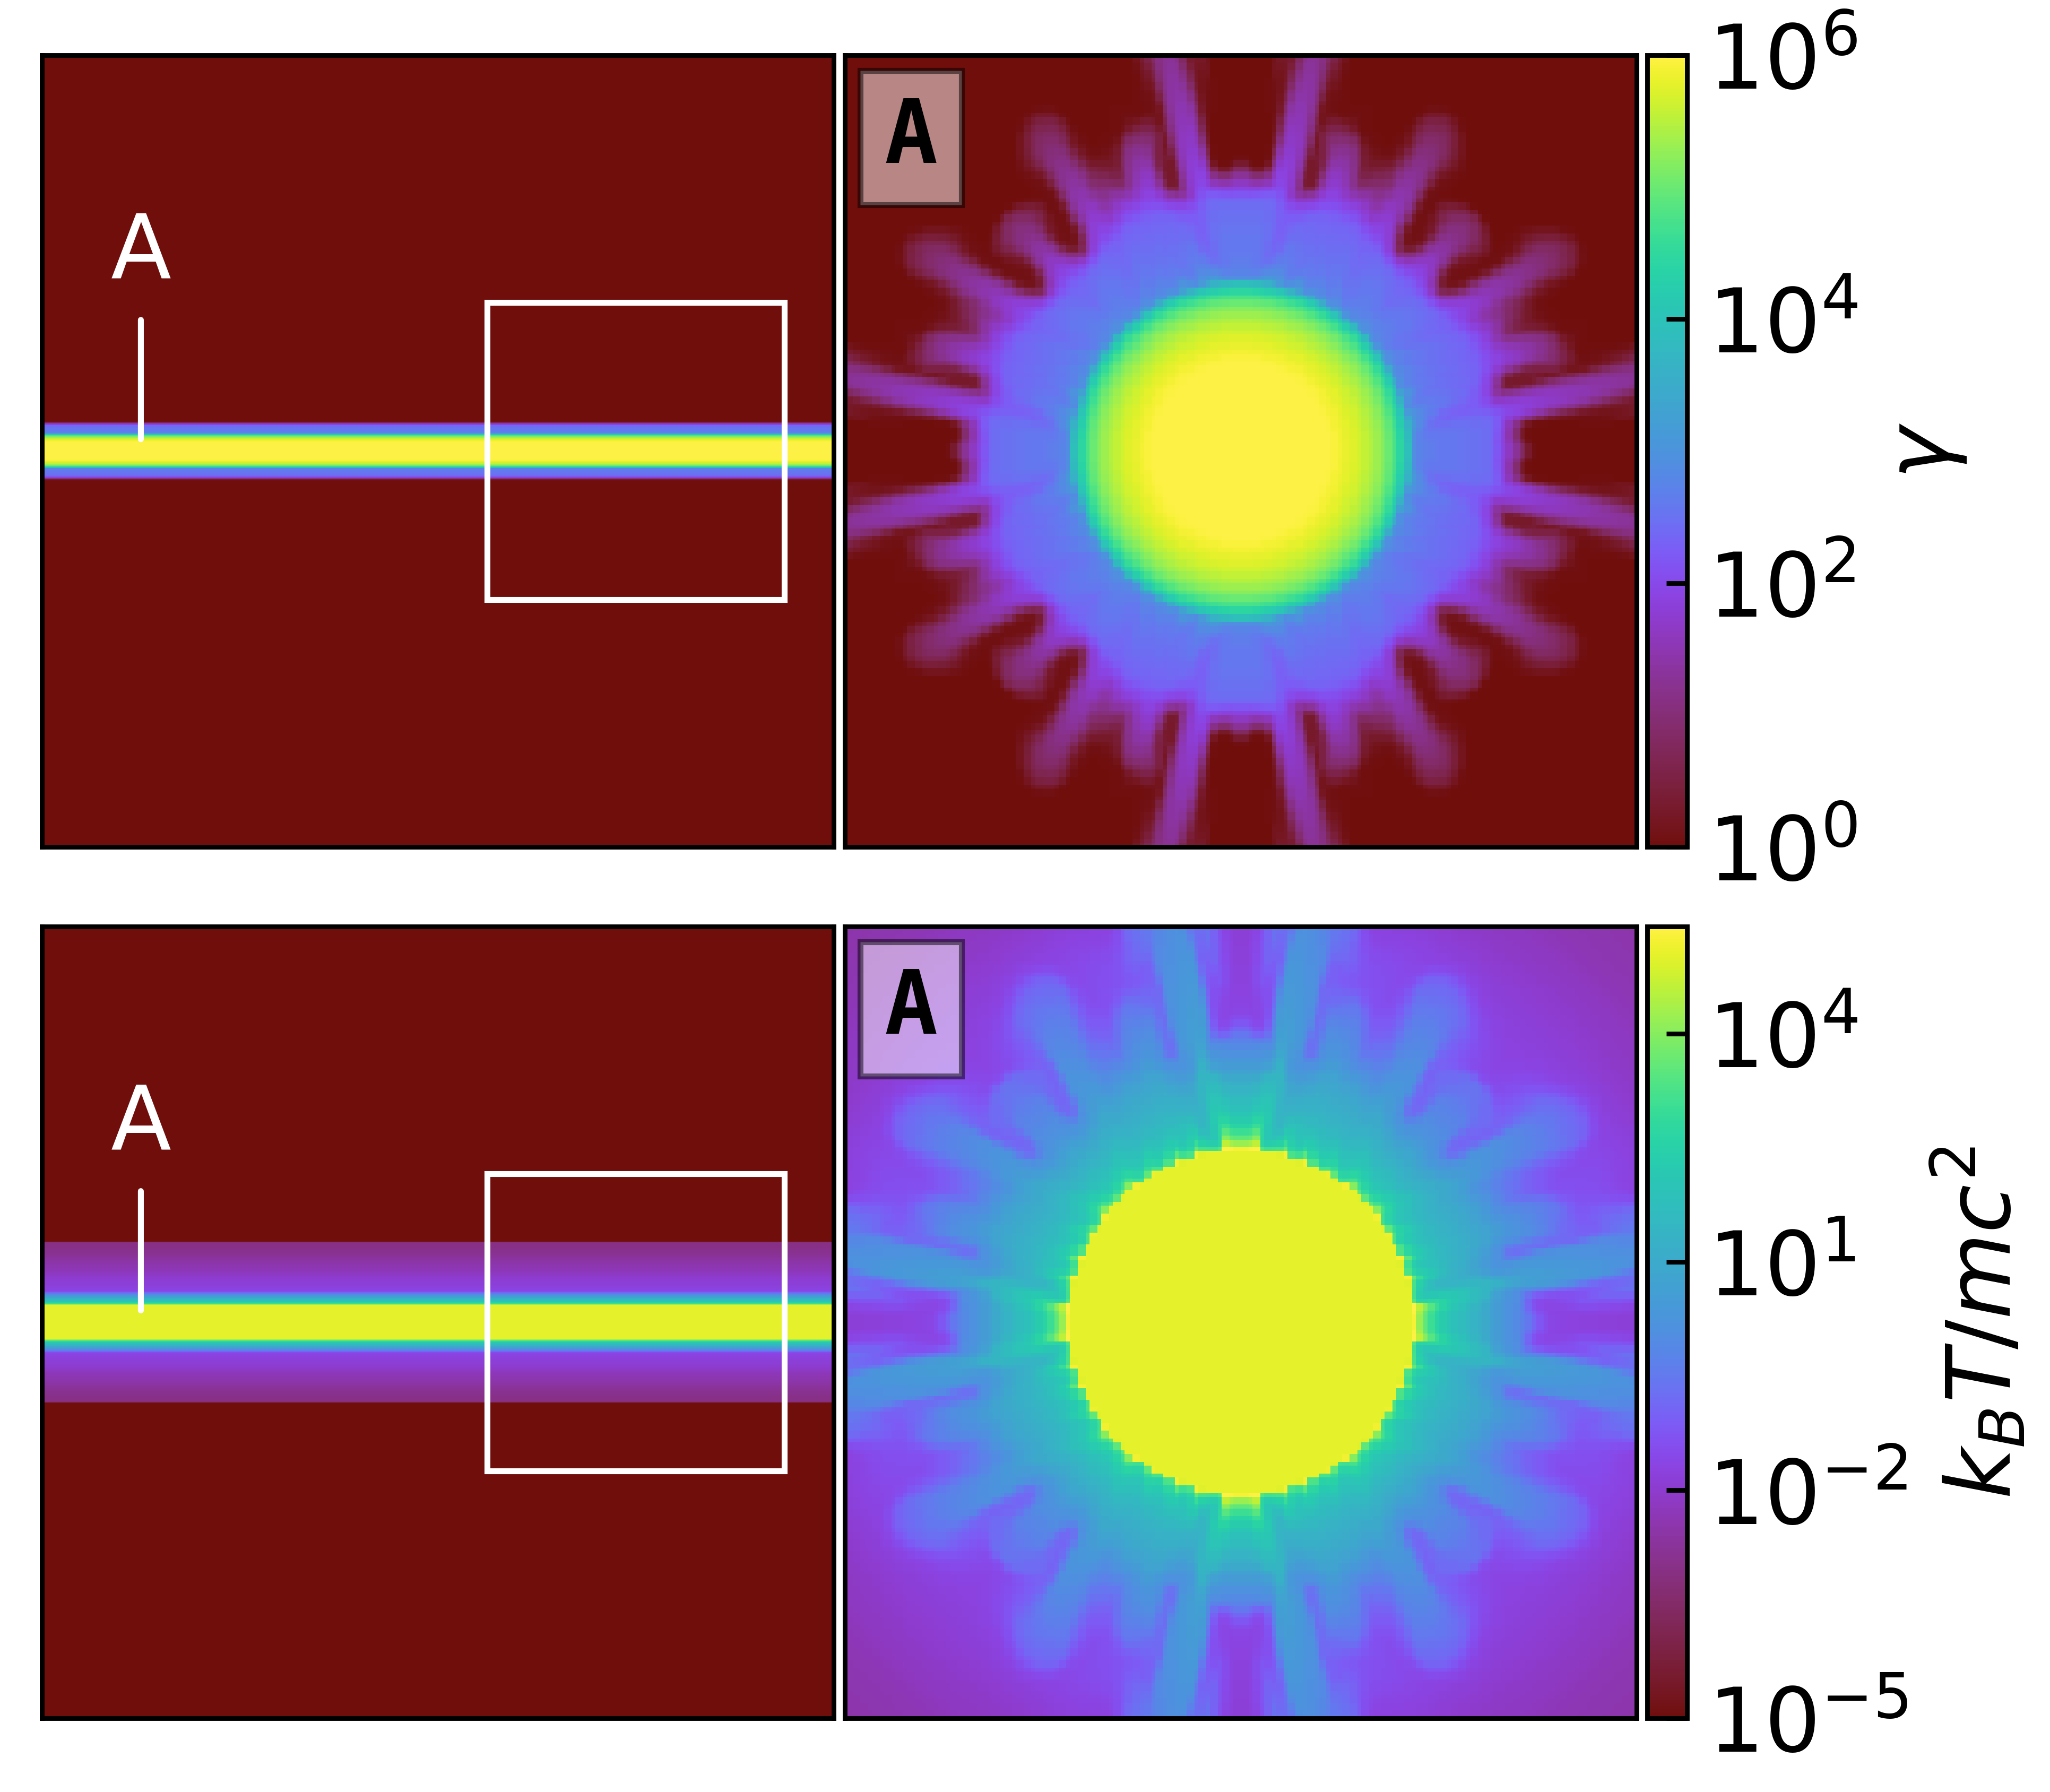
\includegraphics[width=0.45\linewidth]{figures/fig__HorizontalFlowHig.png}
      \label{fig:HorizontalFlowHig} %C
    }
  \subfigure[]
    {
      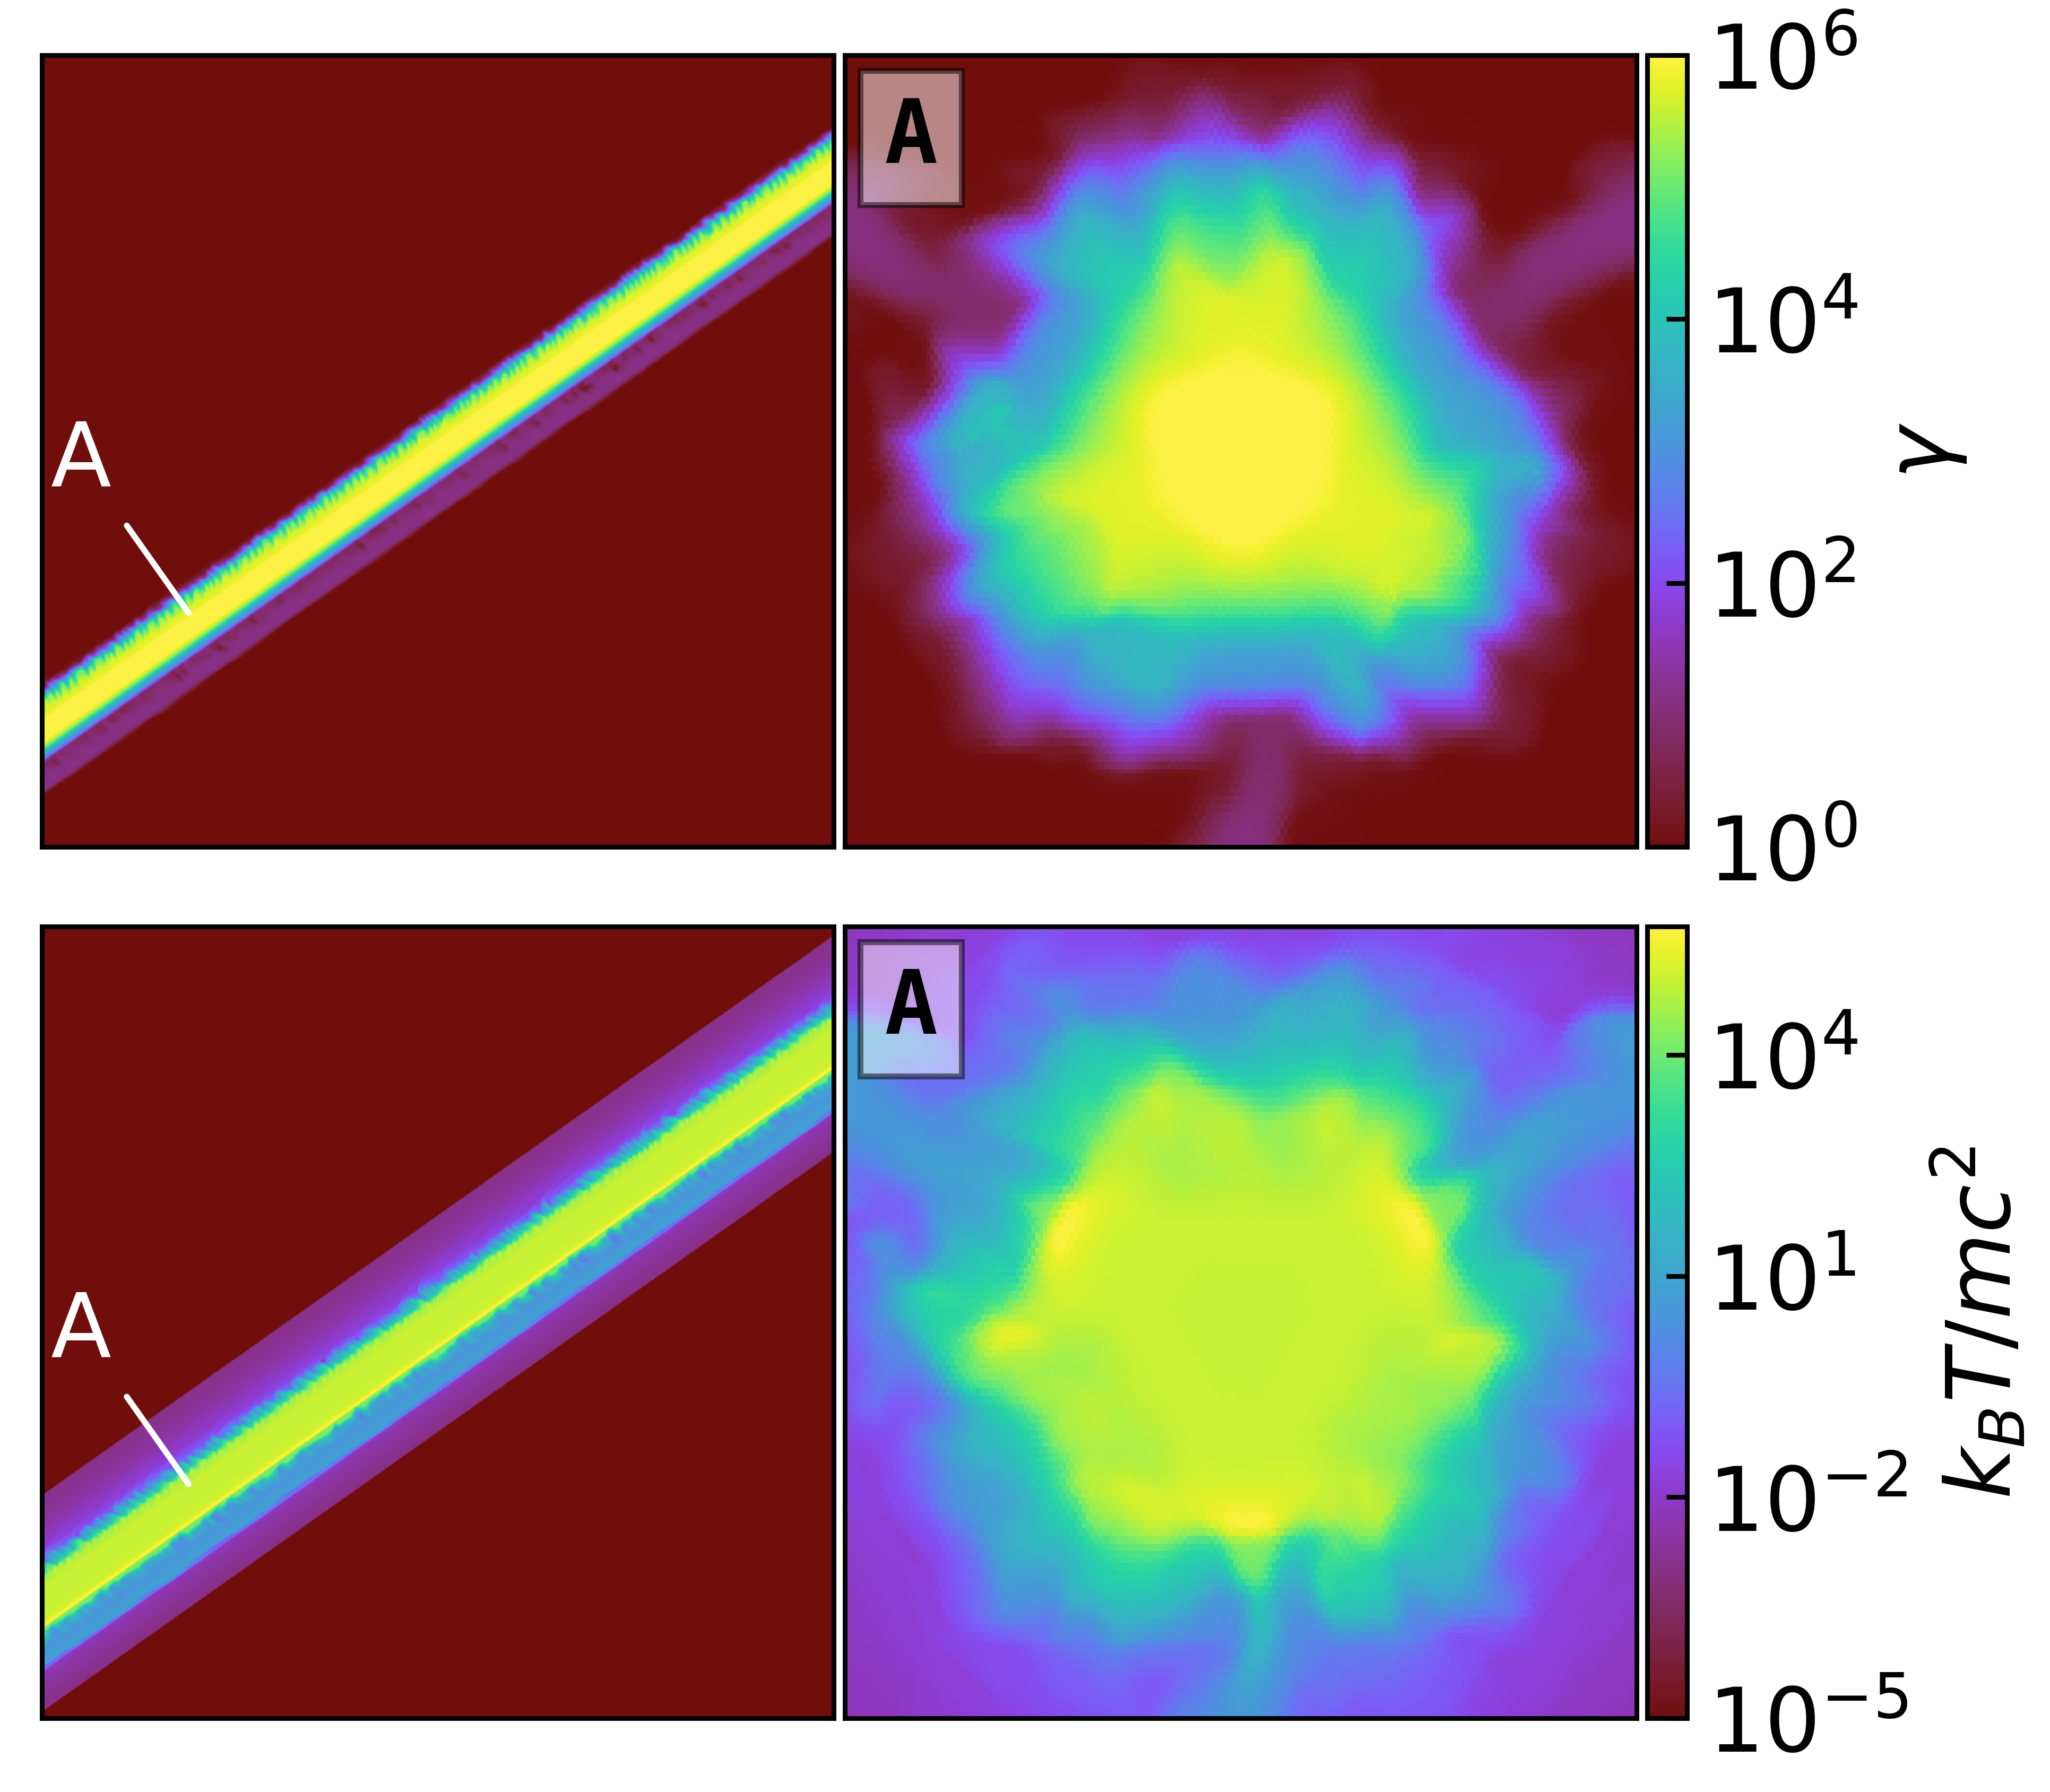
\includegraphics[width=0.45\linewidth]{figures/fig__DiagonalFlowHig.png}
      \label{fig:DiagonalFlowHig} %D
    }
  \caption{
Ultra-relativistic flows propagating along different spatial directions with respect to the grids. In all subfigures (a)--(d), the left and right columns are the longitudinal and transverse slices, respectively. Longitudinal slices are taken through the flow source while the transverse slices are taken through the label `A'. The flow diameter is resolved by 28 cells in (a) and (b) and by 56 cells in (c) and (d). The flow has an extremely high Mach number ($\mathscr{M}\sim 10^{6}$) leaving any instability short of time to develop, and one expects a smooth flow-ambient interface. However, the fuzzy-looking cross-sections in the transverse slices of the oblique flow (right columns in (b) and (d)) suggest that the high-speed flow induces false instability when the flow travels obliquely across Cartesian grids. Increasing the spatial and temporal resolution does not help the numerical solution of an oblique flow to converge to that of a parallel flow.}
  \label{fig:GridEffect}
\end{figure*}






\begin{figure}
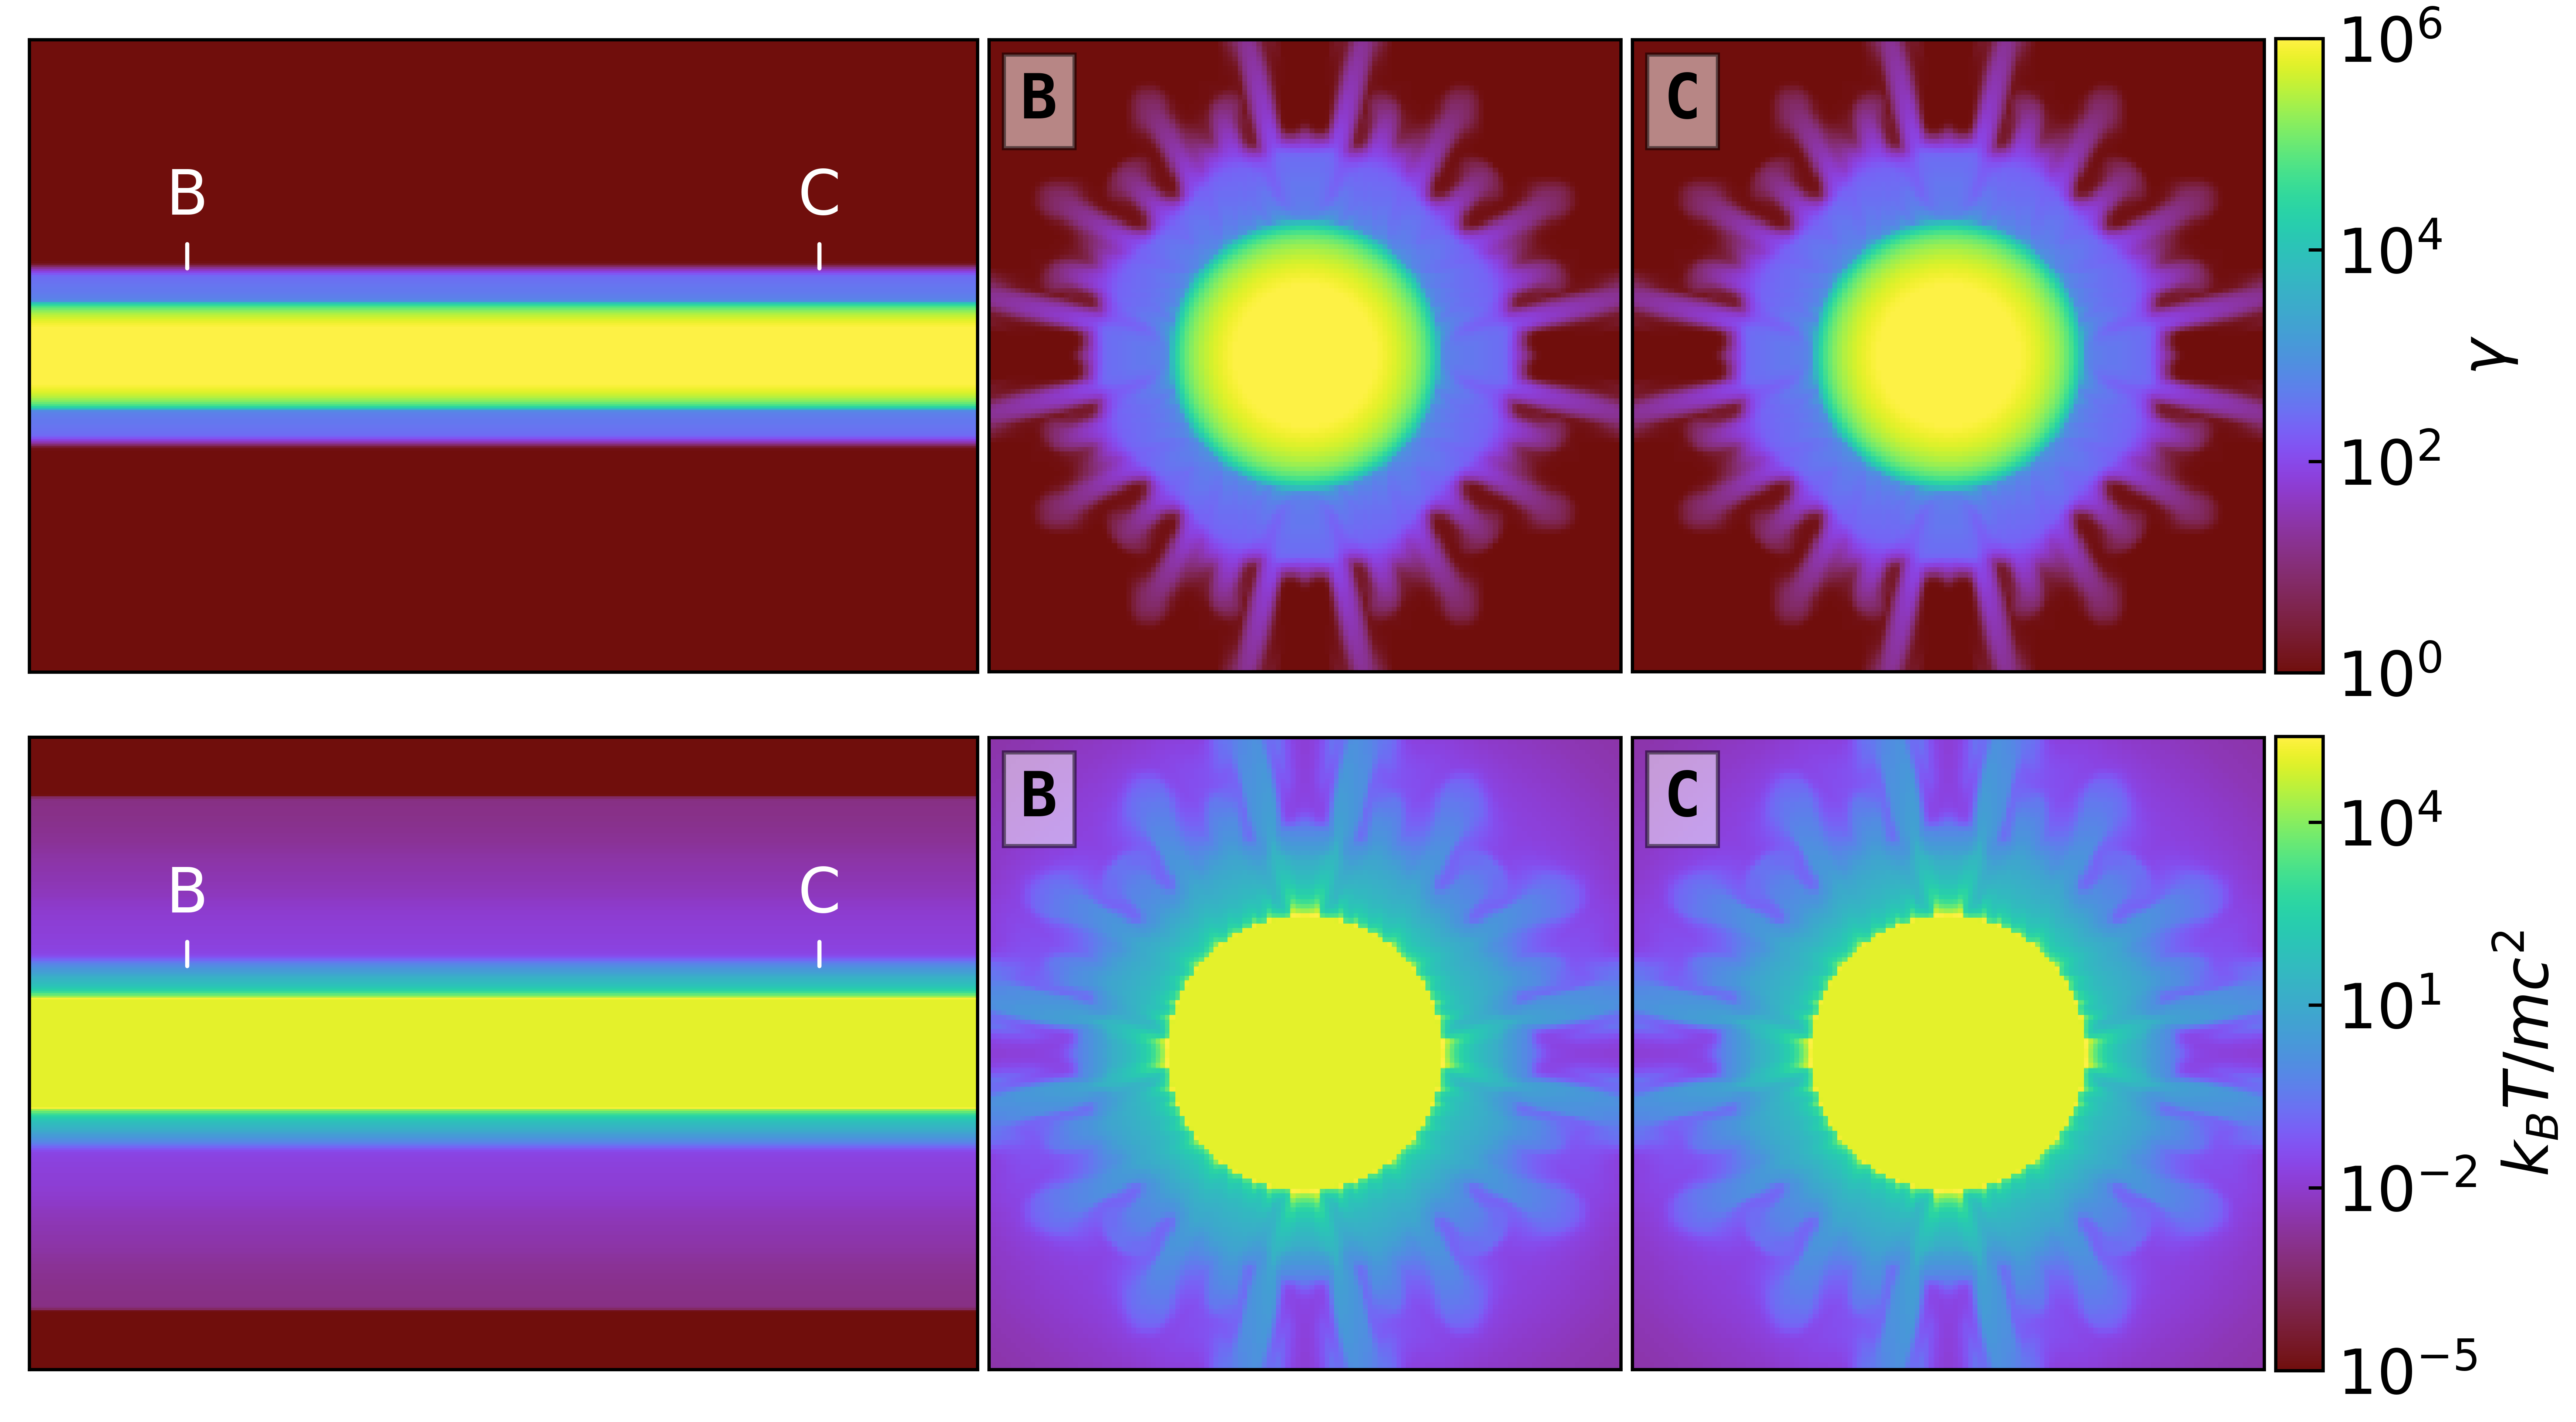
\includegraphics[width=\columnwidth]{figures/fig__HorizontalFlowHigZoomIn.png}
\centering
\caption{Close-up view of the rectangular region in \Cref{fig:HorizontalFlowHig} with longitudinal (first column from the left) and transverse (other columns) slices passing through `B' and `C', respectively. Compared with \Cref{fig:HorizontalFlowHig}, it clearly shows that the finger pattern consists of 2-D flat sheets along the flow.}
\label{fig:HorizontalFlowHigZoomIn}
\end{figure}


